\documentclass[conference,a4paper]{IEEEtran}
%\IEEEoverridecommandlockouts
% The preceding line is only needed to identify funding in the first footnote. If that is unneeded, please comment it out.
\usepackage[T1]{fontenc}
\usepackage[left=1.6cm,right=1.6cm,top=1.9cm,bottom=2.54cm]{geometry}
\usepackage{cite}
\usepackage{amsmath,amssymb,amsfonts,gensymb}
\usepackage{algorithmic}
\usepackage{graphicx}
\usepackage{textcomp}
\usepackage{xcolor}
\usepackage{upgreek}
\usepackage{mhchem}
\usepackage{subcaption}
\usepackage{booktabs}
\usepackage{multirow}
\usepackage{tabularray}
\usepackage{comment}
\usepackage{array}
\usepackage{booktabs}
\usepackage{vcell}
\usepackage{rotating}

\def\BibTeX{{\rm B\kern-.05em{\sc i\kern-.025em b}\kern-.08em
    T\kern-.1667em\lower.7ex\hbox{E}\kern-.125emX}}

    \makeatletter
\newcommand{\linebreakand}{%
  \end{@IEEEauthorhalign}
  \hfill\mbox{}\par
  \mbox{}\hfill\begin{@IEEEauthorhalign}
}
\makeatother

\captionsetup{subrefformat=parens}

\begin{document}

\title{The Evolution of EWOD PCB-Based Digital Microfluidics: Fundamentals, Fabrication, and Applications
}
\begin{comment}
\author{\IEEEauthorblockN{1\textsuperscript{st} Farhan Aizuddin}
\IEEEauthorblockA{\textit{Collaborative Microelectronic Design} \\
\textit{Excellence Centre (CEDEC)} \\
\textit{Universiti Sains Malaysia}\\
Penang, Malaysia \\
farhan\_aizzuddin@student.usm.my}
\and
\IEEEauthorblockN{2\textsuperscript{nd} Asrulnizam Abd. Manaf}
\IEEEauthorblockA{\textit{Collaborative Microelectronic Design} \\
\textit{Excellence Centre (CEDEC)} \\
\textit{Universiti Sains Malaysia}\\
Penang, Malaysia \\
eeasrulnizam@usm.my}
\and
\IEEEauthorblockN{3\textsuperscript{rd} Mohd Shahrimie Mohd Asaari}
\IEEEauthorblockA{\textit{School of Electrical} \\
\textit{and Electronics Engineering} \\
\textit{Universiti Sains Malaysia}\\
Penang, Malaysia\\
mohdshahrimie@usm.my}
\linebreakand
\IEEEauthorblockN{4\textsuperscript{th} Mohamad Adzhar Md Zawawi}
\IEEEauthorblockA{\textit{School of Electrical} \\
\textit{and Electronics Engineering} \\
\textit{Universiti Sains Malaysia}\\
Penang, Malaysia \\
adzhar@usm.my}
\and
\IEEEauthorblockN{5\textsuperscript{th}  Beh Khi Kim}
\IEEEauthorblockA{\textit{Collaborative Microelectronic Design} \\
\textit{Excellence Centre (CEDEC)} \\
\textit{Universiti Sains Malaysia}\\
Penang, Malaysia \\
behkhikim@usm.my
}
\and
\IEEEauthorblockN{6\textsuperscript{th} Beh Khi Poay}
\IEEEauthorblockA{\textit{School of Physics} \\
\textit{Universiti Sains Malaysia}\\
Penang, Malaysia \\
behkhipoay@usm.my}
\linebreakand
}
\end{comment}
\maketitle

\begin{abstract}
Electrowetting-on-dielectric (EWOD) has emerged as a powerful technique for digital microfluidics (DMF), enabling precise manipulation of discrete droplets on a planar surface. Integrating this technology with printed circuit board (PCB) fabrication methods has led to the development of cost-effective, compact, and highly reconfigurable platforms suitable for a wide range of applications. This paper explores the evolution of EWOD PCB-based DMF systems, focusing on their working principles, material stack configurations, and fabrication strategies. The use of multilayer PCBs facilitates complex electrode routing, making high-density, addressable arrays feasible without the need for cleanroom facilities. The application of EWOD PCB-based DMF were higlighted in biomedical and environmental applications, including point-of-care diagnostics, nucleic acid detection, proteomics, and chemical sensing. Despite limitations such as high actuation voltages, resolution constraints, and biofouling, recent advances in materials and system integration continue to enhance performance and functionality. The continued development of EWOD PCB-based DMF holds promise for scalable, portable, and automated lab-on-PCB systems across clinical, industrial, and research domains.
\end{abstract}

\begin{IEEEkeywords}
DMF, EWOD, Lab-on-a-Chip, PCB
\end{IEEEkeywords}

\section{Introduction}
Electrowetting-on-dielectric (EWOD)–based digital microfluidics (DMF) enables programmable manipulation of discrete droplets—such as dispensing, transport, merging, and splitting—using electric fields on a flat substrate as illustrated in Figure \subref{dmf_example}, unlike traditional continuous-flow microfluidics. This eliminates the need for mechanical components like micro-pumps or valves as shown in Figure \subref{microfluidics_example}. The underlying principle is governed by the Young–Lippmann equation, which relates voltage to contact angle modulation \cite{kimPCBbasedDigitalMicrofluidic2024}.

\begin{figure}[h!]
\centering
\begin{subfigure}[b]{0.49\linewidth}
\centering
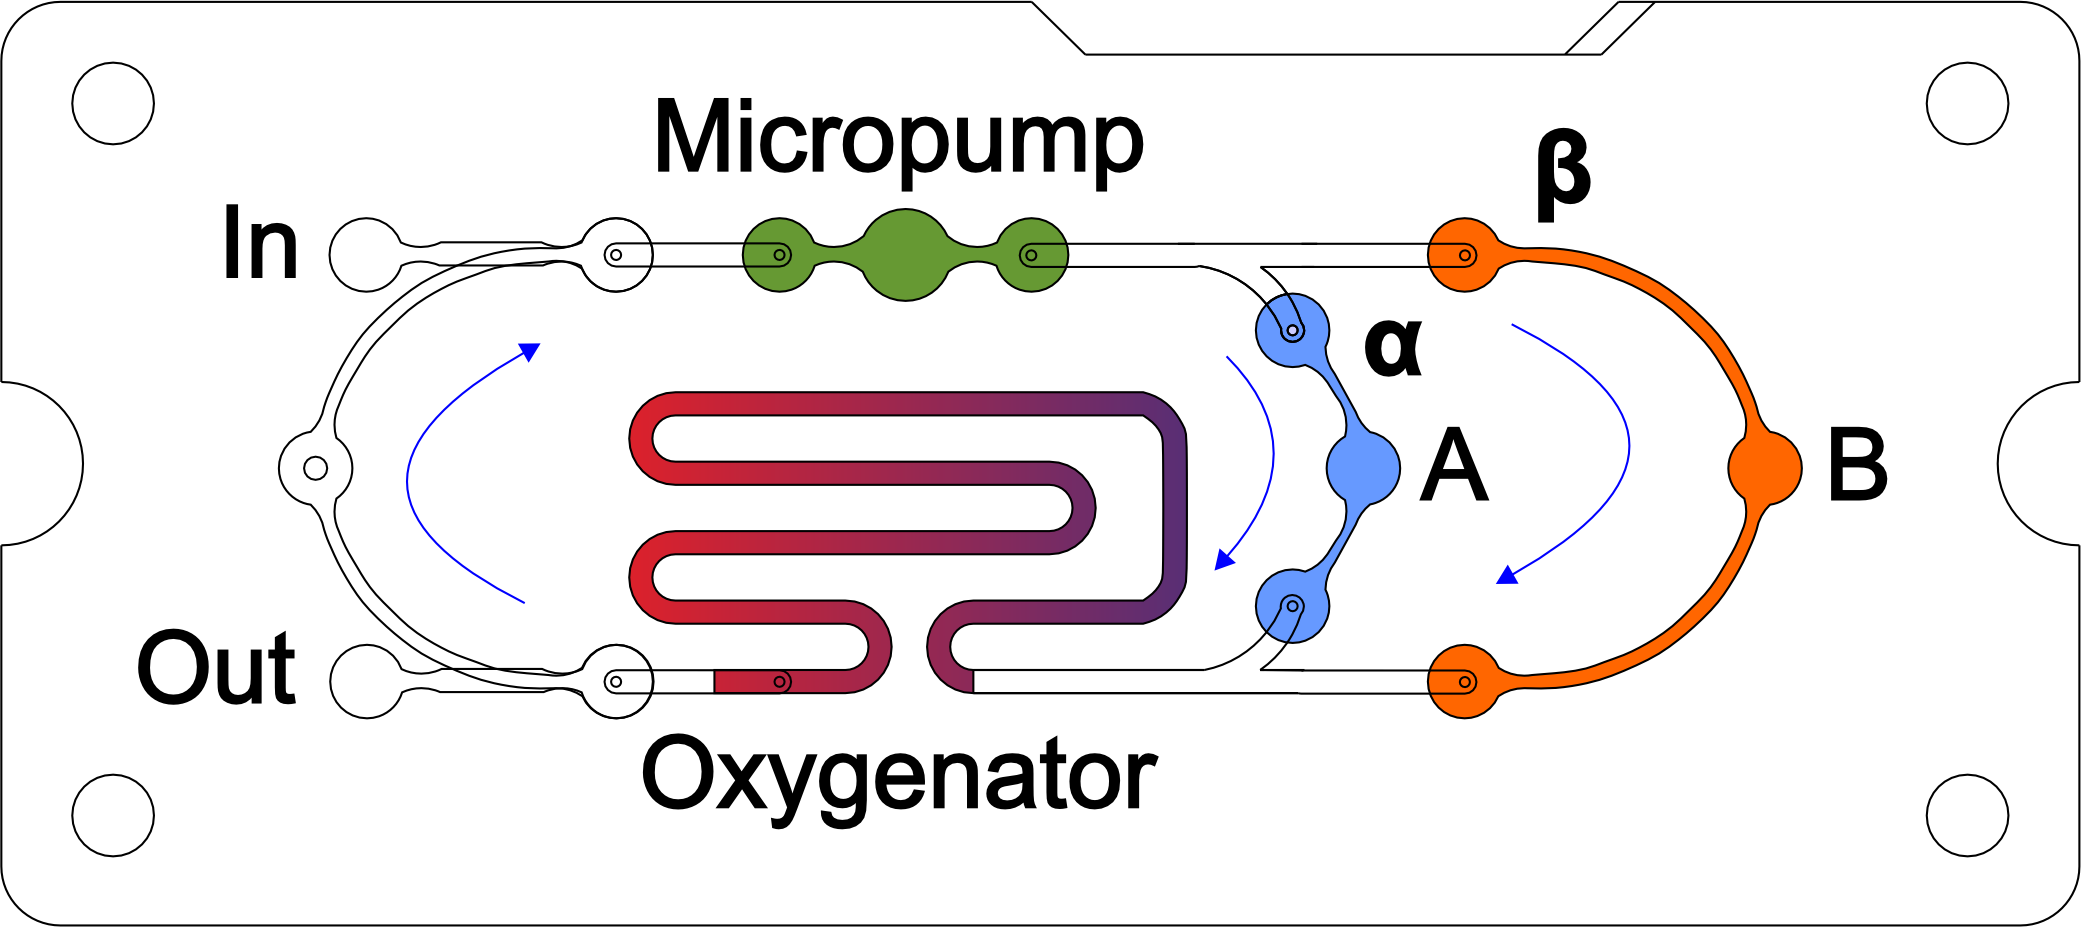
\includegraphics[width=\linewidth]{ExampleMicrofluidics.png}
\caption{}
\label{microfluidics_example}
\end{subfigure}
\begin{subfigure}[b]{0.49\linewidth}
\centering
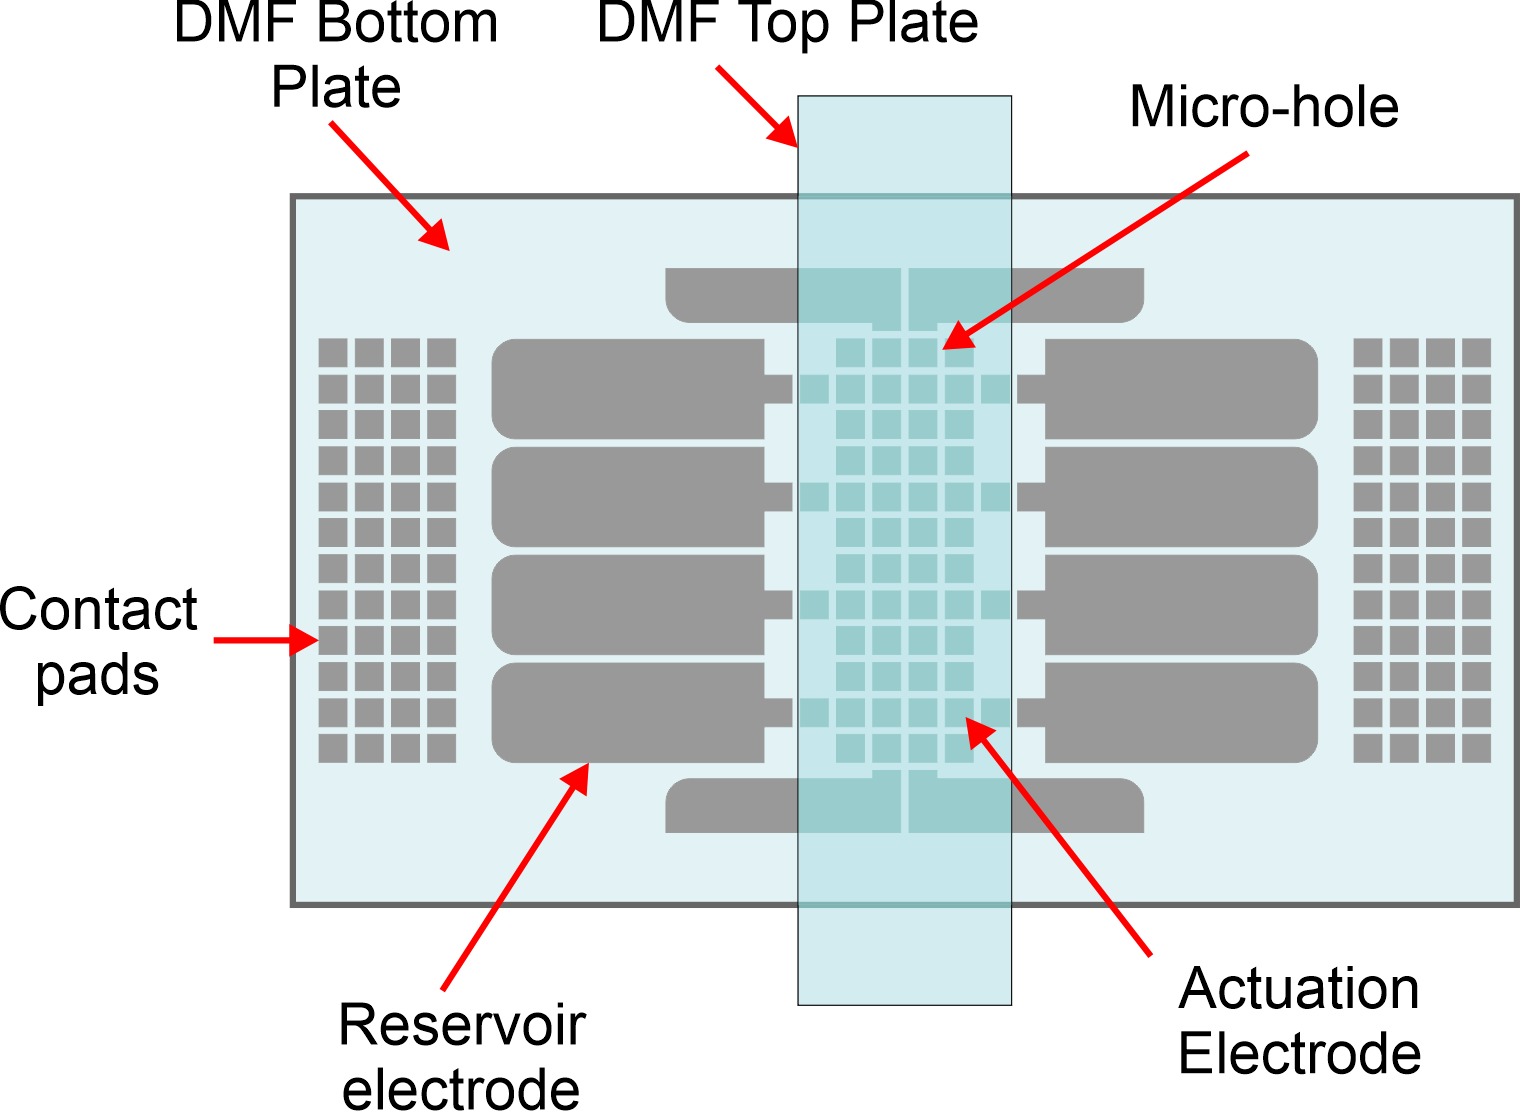
\includegraphics[width=\linewidth]{ExampleDMF.png}
\caption{}
\label{dmf_example}
\end{subfigure}
\caption{Comparison between \subref{microfluidics_example} conventional microfluidics (adapted from \cite{busekDesignCharacterizationModeling2016}) and \subref{dmf_example} EWOD-DMF device (adapted from \cite{pengAllinOneDigitalMicrofluidics2023}).}
\label{microfluidics_vs_dmf}
\end{figure}

Conventional EWOD-DMF systems are typically fabricated on glass or silicon using cleanroom processes \cite{vafaieNumericalSimulationEWOD2019}, which, while precise, are expensive and integration-limited. PCBs present a cost-effective, scalable alternative with mature fabrication methods, multilayer routing, and easy integration with control electronics \cite{jiangongDirectreferencingTwodimensionalarrayDigital2008,sukthangRapidFabricationCloseTyped2020,yiDesignOpenElectrowetting2020}.

This review surveys the evolution of EWOD-DMF platforms, emphasizing PCB-based implementations. It covers foundational EWOD theory, droplet dynamics, electrode design, actuation strategies, applications, and future research directions.\section{Fundamentals of EWOD-based DMF}

\subsection{Principles of EWOD}
The core mechanism behind digital microfluidics (DMF) using electrowetting-on-dielectric (EWOD) is the electrowetting effect—where applying voltage reduces the contact angle of a conductive droplet on a dielectric surface, enhancing wettability by altering interfacial energies at the three-phase contact line (Figure~\ref{ewod_principle}) \cite{royFeedbackBasedAutomated2013,bhattacharjeeMultipleDilutionSample2012,jainDesignFabricationCharacterization2017}.

This behavior is described by the Young–Lippmann equation \cite{jainDesignFabricationCharacterization2017}:
\begin{equation}\label{young_lippmann}
\cos(\theta_{V}) = \cos(\theta_{0}) + \frac{\epsilon_{0}\epsilon_{r} V^{2}}{2\gamma_{LG} d}
\end{equation}
\noindent where $\theta_0$ and $\theta_V$ are the contact angles before and after voltage $V$, $\epsilon_r$ is the dielectric’s permittivity, $\gamma_{LG}$ is the liquid–gas surface tension, and $d$ is the dielectric thickness.

As voltage increases, contact angle decreases quadratically, causing the droplet to spread. By selectively actuating electrodes, localized surface tension gradients move droplets in a programmable fashion—enabling transport, dispensing, merging, and splitting \cite{lovelessCompilingFunctionsDigital2023,jainDesignFabricationCharacterization2017}.

\begin{figure}[h!]
\centering
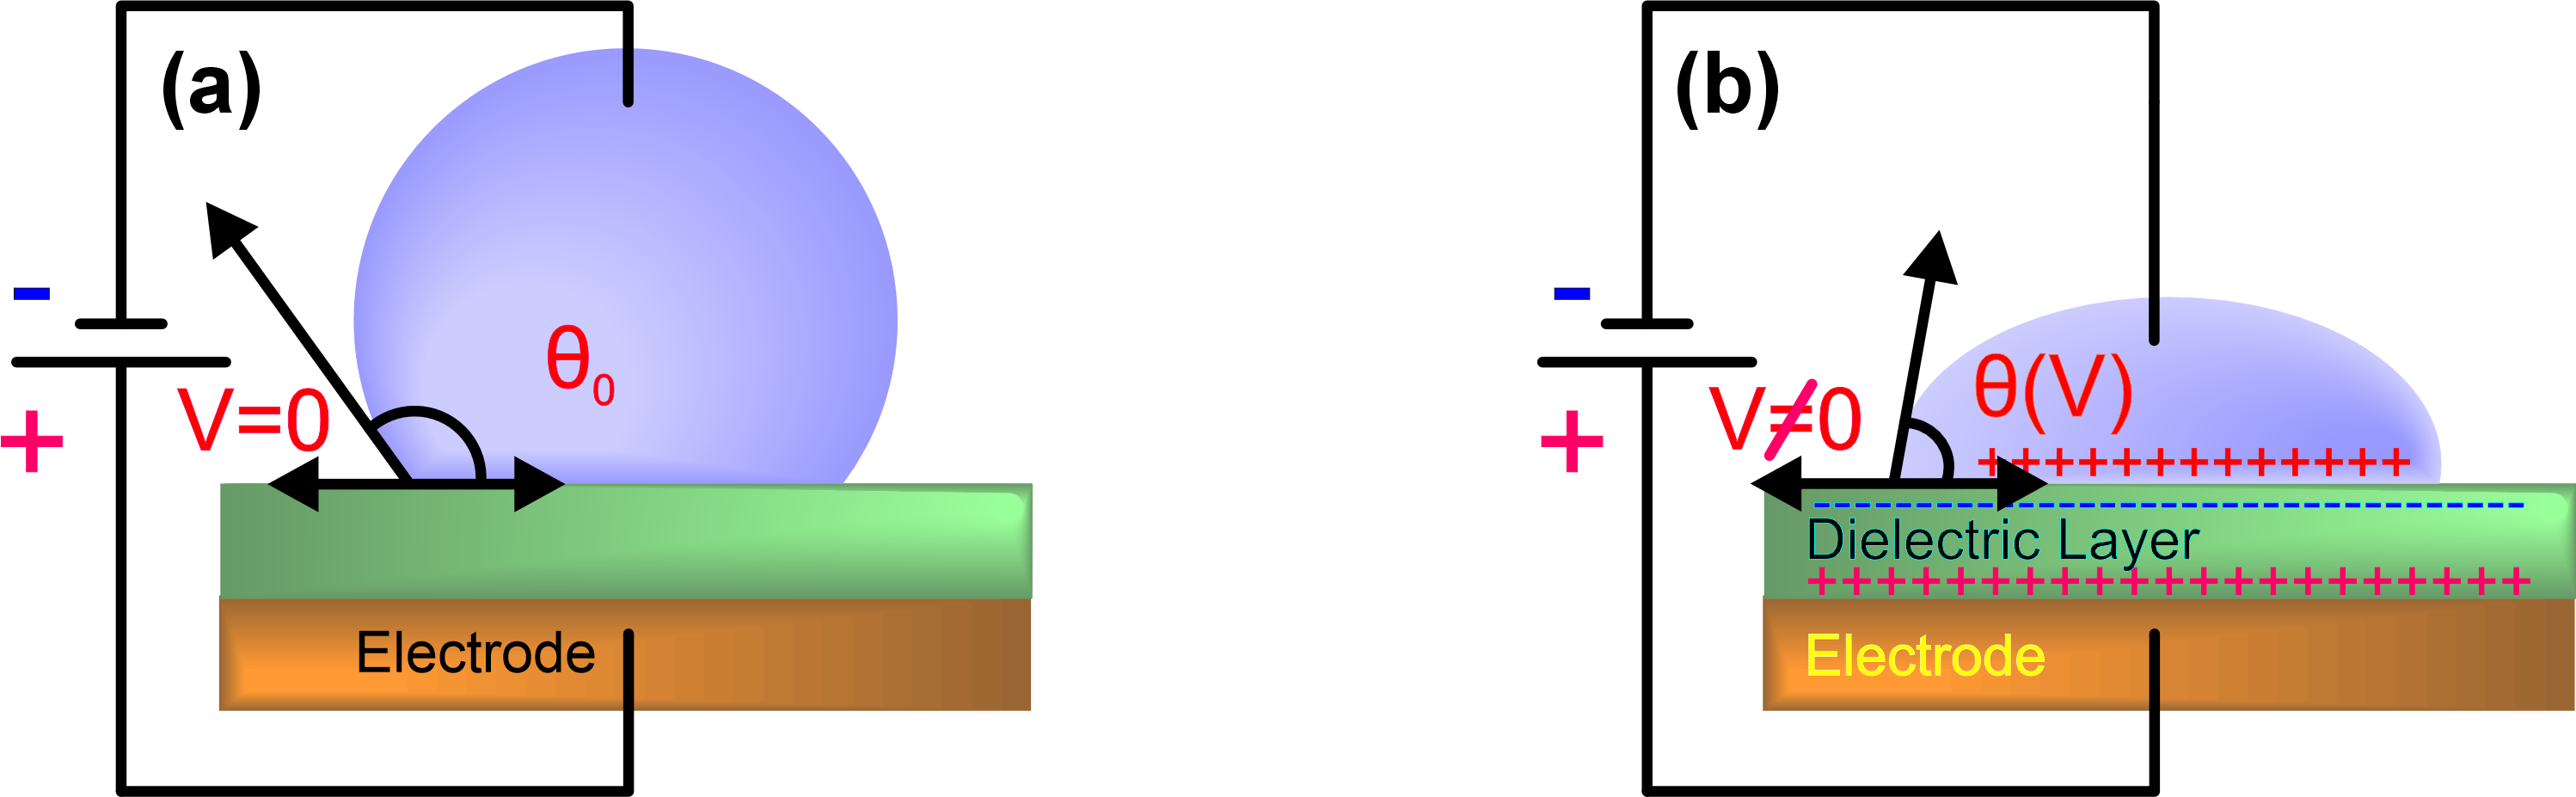
\includegraphics[width=0.85\linewidth]{ContactAngleWhenActuated.png}
\caption{Principle of electrowetting on dielectric (EWOD) for digital microfluidics (DMF) (adapted from \cite{jainEffectElectrodeGeometry2017}).}
\label{ewod_principle}
\end{figure}

As shown in Figure~\ref{ewod_principle}, voltage application reduces the contact angle, inducing droplet movement. The effectiveness of this mechanism is further influenced by the dielectric and hydrophobic layer properties, as well as electrode geometry—all critical for performance, energy efficiency, and robustness.

\subsection{Material Stack Configuration and Fabrication Methods}
The performance and reliability of EWOD PCB-based DMF systems critically depend on the configuration and properties of the material stack used. Each layer in the stack plays a fundamental role in enabling electrowetting functionality while ensuring mechanical stability, chemical resistance, and compatibility with fluid samples \cite{abadianHybridPaperbasedMicrofluidics2017}.

The choice and combination of these materials directly influence the efficiency of electrowetting, the required actuation voltage, and the long-term reliability of the device—particularly under repeated droplet cycling or in bioassay conditions. Table \ref{DMF_materials} outlines commonly used materials for each layer, along with their relevant properties and advantages.

Following material selection, the fabrication process integrates these layers into a functional microfluidic system. Leveraging mature and scalable standard PCB fabrication techniques—such as multilayer routing, etching, solder mask application, and via drilling—enables precise patterning of control electrodes. These techniques make it feasible to construct large-scale electrode arrays with individual addressability at low cost as listed in Table \ref{DMF_process}.

% Table I: Materials
% ===== TABLE I: Materials =====\begin{table}
\begin{table}[h!]
\centering
\caption{Components in EWOD PCB-based DMF}
\label{DMF_materials}
\begin{tblr}{
  width = \linewidth,
  colspec = {Q[237]Q[38]Q[212]Q[38]Q[267]Q[38]Q[79]},
  row{even} = {t},
  row{1} = {c},
  hline{1,11} = {-}{0.08em},
  hline{2} = {1,3,5,7}{},
}
Component &  & Materials &  & Advantage &  & Ref\\
Substrate &  & {\labelitemi\hspace{\dimexpr\labelsep+0.5\tabcolsep}FR4\\\labelitemi\hspace{\dimexpr\labelsep+0.5\tabcolsep}PET\\\labelitemi\hspace{\dimexpr\labelsep+0.5\tabcolsep}Paper} &  & {\labelitemi\hspace{\dimexpr\labelsep+0.5\tabcolsep}Low-cost\\\labelitemi\hspace{\dimexpr\labelsep+0.5\tabcolsep}Multilayer\\\phantom{\labelitemi}\hspace{\dimexpr\labelsep+0.5\tabcolsep}compatible\\\labelitemi\hspace{\dimexpr\labelsep+0.5\tabcolsep}Flexible} &  & \cite{mikhaylovDevelopmentCharacterisationAcoustofluidic2020,abadianHybridPaperbasedMicrofluidics2017}\\
 &  &  &  &  &  & \\
Electrodes &  & {\labelitemi\hspace{\dimexpr\labelsep+0.5\tabcolsep}Copper~\\\labelitemi\hspace{\dimexpr\labelsep+0.5\tabcolsep}CNT~\\\phantom{\labelitemi}\hspace{\dimexpr\labelsep+0.5\tabcolsep}ink} &  & {\labelitemi\hspace{\dimexpr\labelsep+0.5\tabcolsep}Easy~\\\phantom{\labelitemi}\hspace{\dimexpr\labelsep+0.5\tabcolsep}patterning\\\labelitemi\hspace{\dimexpr\labelsep+0.5\tabcolsep}Supports~\\\phantom{\labelitemi}\hspace{\dimexpr\labelsep+0.5\tabcolsep}low-cost\\\phantom{\labelitemi}\hspace{\dimexpr\labelsep+0.5\tabcolsep}printing} &  & \cite{chakrabartyFaulttolerantReconfigurableDigital2010,yafiaUltraportableSmartphoneControlled2015}\\
 &  &  &  &  &  & \\
{Dielectric\\layer} &  & {\labelitemi\hspace{\dimexpr\labelsep+0.5\tabcolsep}PDMS\\\labelitemi\hspace{\dimexpr\labelsep+0.5\tabcolsep}SU-8\\\labelitemi\hspace{\dimexpr\labelsep+0.5\tabcolsep}PE film} &  & {\labelitemi\hspace{\dimexpr\labelsep+0.5\tabcolsep}High~\\\phantom{\labelitemi}\hspace{\dimexpr\labelsep+0.5\tabcolsep}dielectric~\\\phantom{\labelitemi}\hspace{\dimexpr\labelsep+0.5\tabcolsep}constant} &  & \cite{vafaieNumericalSimulationEWOD2019,nardecchia2DDigitalMicrofluidic2015,jinOnetothreeDropletGeneration2021}\\
 &  &  &  &  &  & \\
{Hydrophobic\\layer} &  & {\labelitemi\hspace{\dimexpr\labelsep+0.5\tabcolsep}Teflon-\\\phantom{\labelitemi}\hspace{\dimexpr\labelsep+0.5\tabcolsep}AF\\\labelitemi\hspace{\dimexpr\labelsep+0.5\tabcolsep}Rain-\\\phantom{\labelitemi}\hspace{\dimexpr\labelsep+0.5\tabcolsep}X®\\\labelitemi\hspace{\dimexpr\labelsep+0.5\tabcolsep}CYTOP\\\labelitemi\hspace{\dimexpr\labelsep+0.5\tabcolsep}Silicone\\\phantom{\labelitemi}\hspace{\dimexpr\labelsep+0.5\tabcolsep}oil} &  & {\labelitemi\hspace{\dimexpr\labelsep+0.5\tabcolsep}Reduces~\\\phantom{\labelitemi}\hspace{\dimexpr\labelsep+0.5\tabcolsep}pinning\\\labelitemi\hspace{\dimexpr\labelsep+0.5\tabcolsep}Enhances~\\\phantom{\labelitemi}\hspace{\dimexpr\labelsep+0.5\tabcolsep}mobility} &  & \cite{yiDesignOpenElectrowetting2020,nardecchia2DDigitalMicrofluidic2015,haleElectrowettingbasedMicrofluidicOperations2017}\\
 &  &  &  &  &  & \\
Fiiller fluid &  & {\labelitemi\hspace{\dimexpr\labelsep+0.5\tabcolsep}Silicone~\\\phantom{\labelitemi}\hspace{\dimexpr\labelsep+0.5\tabcolsep}oil\\\labelitemi\hspace{\dimexpr\labelsep+0.5\tabcolsep}Mineral~\\\phantom{\labelitemi}\hspace{\dimexpr\labelsep+0.5\tabcolsep}oil} &  & {\labelitemi\hspace{\dimexpr\labelsep+0.5\tabcolsep}Reduces~\\\phantom{\labelitemi}\hspace{\dimexpr\labelsep+0.5\tabcolsep}applied~\\\phantom{\labelitemi}\hspace{\dimexpr\labelsep+0.5\tabcolsep}voltage\\\labelitemi\hspace{\dimexpr\labelsep+0.5\tabcolsep}Prevents\\\phantom{\labelitemi}\hspace{\dimexpr\labelsep+0.5\tabcolsep}evaporation} &  & \cite{sukthangRapidFabricationCloseTyped2020}
\end{tblr}
\end{table}
% ===== TABLE II: Fabrication Process =====
\begin{table}[h!]
\centering
\caption{Fabrication process for EWOD PCB-based DMF}
\label{DMF_process}
\begin{tblr}{
  width = \linewidth,
  colspec = {Q[181]Q[25]Q[423]Q[25]Q[198]Q[25]Q[54]},
  row{1} = {c},
  cell{2}{7} = {c,t},
  cell{3}{7} = {c,t},
  cell{4}{7} = {c,t},
  hline{1,5} = {-}{0.08em},
  hline{2} = {1,3,5,7}{},
}
{Fabrication\\Process}  &  & {Fabrication\\Methods}                                                                                                                                                                            &  & Advantage                                  &  & Ref. \\
{Standard PCB\\process} &  & {Design, etching, solder mask,vias}                                                                                                                                                             &  & {Scalable, multilayer\\routing possible}   &  & \cite{wuMicrofluidicPrintedCircuit2011,haleElectrowettingbasedMicrofluidicOperations2017,yiDesignOpenElectrowetting2020,jiangongDirectreferencingTwodimensionalarrayDigital2008}     \\
                        &  &                                                                                                                                                                                                   &  &                                            &  &      \\
Rapid Prototyping       &  & {Screen printing, \\Inkjet printing, \\Graphic spraying, \\ PCB routing machine (milling), \\Coplanar design, \\Simplified dielectric/hydrophobic deposition, \\Top-plate integration} &  & {Low-cost, ideal for\\disposable devices} &  & \cite{abadianHybridPaperbasedMicrofluidics2017,haleElectrowettingbasedMicrofluidicOperations2017,royNewDesignDual2012,ullahDropletActuationEnhancement2024,jinOnetothreeDropletGeneration2021}
\end{tblr}
\end{table}

\subsection{Electrode Design Considerations}
Electrode design is central to the performance of EWOD-based digital microfluidic (DMF) systems, as it governs the electric field distribution and thus the precision of droplet operations like transport, dispensing, splitting, and merging. Key design parameters—such as droplet volume, electrode shape and size, spacing, actuation voltage, and force symmetry—affect not only droplet control but also fabrication complexity and layout efficiency \cite{guanStrippedElectrodeBased2020,wuResearchProgressElectrode2023,chenDigitalMicrofluidicsChip2015,dimovElectrowettingbasedDigitalMicrofluidics2020,sukthangRapidFabricationCloseTyped2020,abadianHybridPaperbasedMicrofluidics2017,al-lababidiMinimumMovableDroplet2023,huOptimizationElectrodeShape2024,sohailJigsawElectrodeDesign2019}.

To address varying operational and fabrication needs, a range of electrode geometries have been developed, from basic square shapes to interdigitated, crescent, stripped, dumbbell, and jigsaw designs. Each offers trade-offs in terms of transport efficiency, droplet compatibility, and ease of integration. A comparative summary is provided in Table~\ref{electrode_comparison}, adapted from Wu et al. \cite{wuResearchProgressElectrode2023}.

\begin{table*}[htbp!]
\centering
\caption{Comparison of different electrode designs for EWOD-based DMF systems \cite{wuResearchProgressElectrode2023}}
\label{electrode_comparison}
\begin{tblr}{
  width = \linewidth,
  colspec = {Q[121]Q[25]Q[138]Q[25]Q[281]Q[25]Q[315]},
  row{even} = {t},
  row{1} = {c},
  hline{1,13} = {-}{0.08em},
  hline{2} = {1,3,5,7}{},
}
Electrode type &  & Operation &  & Advantages &  & Limitations\\
Square &  & {\labelitemi\hspace{\dimexpr\labelsep+0.5\tabcolsep}Transporting\\\labelitemi\hspace{\dimexpr\labelsep+0.5\tabcolsep}Dispensing} &  & {\labelitemi\hspace{\dimexpr\labelsep+0.5\tabcolsep}Simple\\\labelitemi\hspace{\dimexpr\labelsep+0.5\tabcolsep}Supports fundamental DMF~\\\phantom{\labelitemi}\hspace{\dimexpr\labelsep+0.5\tabcolsep}operations} &  & {\labelitemi\hspace{\dimexpr\labelsep+0.5\tabcolsep}Limited to fixed droplet sizes~\\\labelitemi\hspace{\dimexpr\labelsep+0.5\tabcolsep}Slow transport\\\labelitemi\hspace{\dimexpr\labelsep+0.5\tabcolsep}Droplet stranding risk}\\
 &  &  &  &  &  & \\
Interdigitated &  & {\labelitemi\hspace{\dimexpr\labelsep+0.5\tabcolsep}Transporting\\\labelitemi\hspace{\dimexpr\labelsep+0.5\tabcolsep}Dispensing} &  & {\labelitemi\hspace{\dimexpr\labelsep+0.5\tabcolsep}Provides continuous transport\\\labelitemi\hspace{\dimexpr\labelsep+0.5\tabcolsep}Suitable for various droplet sizes} &  & {\labelitemi\hspace{\dimexpr\labelsep+0.5\tabcolsep}Fabrication sensitivity\\\labelitemi\hspace{\dimexpr\labelsep+0.5\tabcolsep}Low PCB resolution hinders precision}\\
 &  &  &  &  &  & \\
Crescent &  & \labelitemi\hspace{\dimexpr\labelsep+0.5\tabcolsep}Transporting &  & {\labelitemi\hspace{\dimexpr\labelsep+0.5\tabcolsep}Faster droplet motion\\\labelitemi\hspace{\dimexpr\labelsep+0.5\tabcolsep}Efficient splitting\\\labelitemi\hspace{\dimexpr\labelsep+0.5\tabcolsep}Reduced actuation voltage} &  & \labelitemi\hspace{\dimexpr\labelsep+0.5\tabcolsep}Uni-directional movement\\
 &  &  &  &  &  & \\
Stripped &  & {\labelitemi\hspace{\dimexpr\labelsep+0.5\tabcolsep}Transporting\\\labelitemi\hspace{\dimexpr\labelsep+0.5\tabcolsep}Splitting} &  & \labelitemi\hspace{\dimexpr\labelsep+0.5\tabcolsep}Precise dispensing &  & {\labelitemi\hspace{\dimexpr\labelsep+0.5\tabcolsep}Best suited for closed EWOD~\\\phantom{\labelitemi}\hspace{\dimexpr\labelsep+0.5\tabcolsep}configuration}\\
 &  &  &  &  &  & \\
Dumbbell &  & \labelitemi\hspace{\dimexpr\labelsep+0.5\tabcolsep}Dispensing &  & {\labelitemi\hspace{\dimexpr\labelsep+0.5\tabcolsep}Consistent droplet volume\\\labelitemi\hspace{\dimexpr\labelsep+0.5\tabcolsep}Enhanced tail control} &  & \labelitemi\hspace{\dimexpr\labelsep+0.5\tabcolsep}Limited flexibility in dynamic layouts\\
 &  &  &  &  &  & \\
Jigsaw &  & \labelitemi\hspace{\dimexpr\labelsep+0.5\tabcolsep}Transporting &  & \labelitemi\hspace{\dimexpr\labelsep+0.5\tabcolsep}Simplifies 2D addressing &  & {\labelitemi\hspace{\dimexpr\labelsep+0.5\tabcolsep}Needed custom layout\\\labelitemi\hspace{\dimexpr\labelsep+0.5\tabcolsep}Prone to force asymmetry}
\end{tblr}
\end{table*}

Overall, electrode selection should be application-specific, guided by the intended DMF operation, desired resolution, and fabrication limitations. These findings underscore the importance of aligning design choices with operational and manufacturing constraints to ensure robust droplet control in DMF platforms.
\section{Applications And Implementations}
EWOD PCB-based digital microfluidics (DMF) offers miniaturization, programmability, and precise droplet control, making it ideal for biomedical and diagnostic applications \cite{howladarDesignAutomationTesting2020,dasPaperbasedMicrofluidicDevices2022}. In point-of-care (POC) diagnostics, these platforms enable rapid, multiplexed testing from sample prep to detection \cite{yafiaHighPrecisionControl2013}. Beyond clinical use, EWOD systems have been applied in airborne particle sampling \cite{chakrabartyFaulttolerantReconfigurableDigital2010,jebrailDigitalMicrofluidicsVersatile2012}, and chemical sensing of mercury(II), ammonia, and nitrite in food.

EWOD’s droplet-level control supports on-demand chemical synthesis \cite{chengRecentDesignApplication2025} and complete pipelines for food safety testing \cite{ullahDropletActuationEnhancement2024}. Optical applications include tunable liquid lenses, micromirrors, and solar concentrators \cite{samadDesignFabricationElectrode2015,wuResearchProgressElectrode2023}, along with e-paper and dye laser technologies \cite{garci-sanchezFundamentalsElectrowettingApplications2011,jebrailDigitalMicrofluidicsVersatile2012}.

For thermal regulation, EWOD droplets target hotspots for local cooling \cite{howellModelingSimulationDroplet2010}, and are being explored in electrowetting heat pipes (EHPs) \cite{haleElectrowettingbasedMicrofluidicOperations2017}. Novel uses include liquid-state FETs \cite{garci-sanchezFundamentalsElectrowettingApplications2011}, wafer transport via microbelt conveyors \cite{abdelgawadDigitalRevolutionNew2009}, and filament rheometry \cite{trolsLowcostViscositySensor2016}.

EWOD also supports energy harvesting, microswitches, and bioinspired coatings for diagnostics \cite{kanitthamniyomMagneticDigitalMicrofluidics2019}, with applications in regenerative medicine such as mitochondria transfer \cite{wuResearchProgressElectrode2023}. PCB integration enables embedded sensors and heaters, driving compact, automated, multifunctional DMF systems \cite{wuMicrofluidicPrintedCircuit2011}.

\section{Challenges and Future Works}
EWOD PCB-based digital microfluidics (DMF) use low-cost, scalable PCB fabrication to enable reconfigurable, disposable platforms for 2D droplet control. Multilayer routing supports complex electrode arrays without the expense of cleanroom processes, while screen printing, inkjet, and milling simplify prototyping. Compatible dielectric and hydrophobic materials—such as PDMS, SU-8, Parafilm M, CYTOP, Teflon-AF, and cooking oils—offer affordable, biocompatible options for varied applications.

Challenges include rough PCB surfaces that demand higher voltages or oil immersion for reliable actuation \cite{jiangongDirectreferencingTwodimensionalarrayDigital2008}, limits on feature miniaturization below 500 $\micro$m \cite{abadianHybridPaperbasedMicrofluidics2017}, and biofouling in protein assays \cite{dimovElectrowettingbasedDigitalMicrofluidics2020}. High-voltage needs reduce portability \cite{barmanElectrowettingondielectricEWODCurrent2020}, and open-type DMF struggles with splitting or handling viscous/harsh fluids \cite{yafiaUltraportableSmartphoneControlled2015,pengFingerpoweredElectrophoreticTransport2016}.

Nonetheless, ongoing innovations in materials and fabrication are expanding the reach of PCB-based DMF in biomedical, environmental, and industrial domains.
\section{Conclusion}
The evolution of electrowetting-on-dielectric (EWOD) platforms integrated with printed circuit board (PCB) technology represents a significant step toward democratizing digital microfluidics. Leveraging the low cost, scalability, and design flexibility of PCB fabrication, these systems offer a viable path to compact, disposable, and reconfigurable microfluidic solutions. Their demonstrated applications span a broad spectrum—from point-of-care diagnostics and nucleic acid amplification to environmental sensing, optical systems, and electronics cooling—underscoring their versatility. While technical challenges remain, including surface roughness, high actuation voltages, and biofouling, ongoing research and material innovations continue to overcome these barriers. As EWOD PCB-based DMF matures, it is poised to become a cornerstone technology for next-generation lab-on-a-chip platforms, particularly in resource-limited and decentralized settings.

\section*{Acknowledgment}
The authors gratefully acknowledge the support from the Ministry of Higher Education Malaysia for Fundamental Research Grant Scheme with Project Code: FRGS/1/2022/TK0/USM/02/10.

\bibliographystyle{IEEEtran}
\bibliography{Literature}
\end{document}
